\documentclass[11pt]{scrartcl}
\usepackage[T1]{fontenc}
\usepackage[a4paper, left=3cm, right=2cm, top=2cm, bottom=2cm]{geometry}
\usepackage[activate]{pdfcprot}
\usepackage[ngerman]{babel}
\usepackage[parfill]{parskip}
\usepackage[utf8]{inputenc}
\usepackage[math]{kurier}
\usepackage{amsmath}
\usepackage{amssymb}
\usepackage{xcolor}
\usepackage{epstopdf}
\usepackage{txfonts}
\usepackage{fancyhdr}
\usepackage{graphicx}
\usepackage{prettyref}
\usepackage{hyperref}
\usepackage{eurosym}
\usepackage{setspace}
\usepackage{units}
\usepackage{eso-pic,graphicx}
\usepackage{icomma}
\usepackage{pdfpages}

\definecolor{darkblue}{rgb}{0,0,.5}
\hypersetup{pdftex=true, colorlinks=true, breaklinks=false, linkcolor=black, menucolor=black, urlcolor=darkblue}



\setlength{\columnsep}{2cm}


\newcommand{\arcsinh}{\mathrm{arcsinh}}
\newcommand{\asinh}{\mathrm{arcsinh}}
\newcommand{\ergebnis}{\textcolor{red}{\mathrm{Ergebnis}}}
\newcommand{\fehlt}{\textcolor{red}{Hier fehlen noch Inhalte.}}
\newcommand{\betanotice}{\textcolor{red}{Diese Aufgaben sind noch nicht in der Übung kontrolliert worden. Es sind lediglich meine Überlegungen und Lösungsansätze zu den Aufgaben. Es können Fehler enthalten sein!!! Das Dokument wird fortwährend aktualisiert und erst wenn das \textcolor{black}{beta} aus dem Dateinamen verschwindet ist es endgültig.}}
\newcommand{\half}{\frac{1}{2}}
\renewcommand{\d}{\, \mathrm d}
\newcommand{\punkte}{\textcolor{white}{xxxxx}}
\newcommand{\p}{\, \partial}
\newcommand{\dd}[1]{\item[#1] \hfill \\}

\renewcommand{\familydefault}{\sfdefault}
\renewcommand\thesection{}
\renewcommand\thesubsection{}
\renewcommand\thesubsubsection{}


\newcommand{\themodul}{Messtechnik}
\newcommand{\thetutor}{Prof. Helsper}
\newcommand{\theuebung}{Übungsklausur 2}

\pagestyle{fancy}
\fancyhead[L]{\footnotesize{C. Hansen}}
\chead{\thepage}
\rhead{}
\lfoot{}
\cfoot{}
\rfoot{}

\title{\themodul{}, \theuebung{}, \thetutor}


\author{Christoph Hansen \\ {\small \href{mailto:chris@university-material.de}{chris@university-material.de}} }

\date{}


\begin{document}

\maketitle

Dieser Text ist unter dieser \href{http://creativecommons.org/licenses/by-nc-sa/4.0/}{Creative Commons} Lizenz veröffentlicht.

\textcolor{red}{Ich erhebe keinen Anspruch auf Vollständigkeit oder Richtigkeit. Falls ihr Fehler findet oder etwas fehlt, dann meldet euch bitte über den Emailkontakt.}

\tableofcontents


\newpage



\section{Aufgabe 1}

Die richtigen Antworten sind:


\begin{center}
	\begin{tabular}{c|c|c|c|c|c|c|c}
		1 & 2 & 3 & 4 & 5 & 6 & 7 & 8 \\ 
		\hline a,c & b & c & a & b & b,c & b & c \\  
	\end{tabular} 
\end{center}


\section{Aufgabe 2}


\subsection*{a)}

\begin{align*}
f = \frac{1}{T} = \frac{1}{\unit[4]{ms}} = \unit[250]{Hz}
\end{align*}


\subsection*{b)}

\begin{align*}
I^2 &= \frac{1}{4} \left[ 20^2 \cdot 2 + (-40)^2 \cdot 2 \right] = \unit[1000]{\mu A^2} \\
I &= \unit[31,6]{\mu A}
\end{align*}


\subsection*{c)}

Man kann aus dem Diagramm erkennen, das $I = \unit[10]{\mu A}$ gilt.


\subsection*{d)}

\paragraph{Schritt 1}

Wechselspannungseinkopplung, das macht den Gleichtaktanteil zu 0.

\paragraph{Schritt 2}

Gleichrichtung

\paragraph{Schritt 3}

arithmetischer Mittelwert $\unit[30]{\mu A}$

\paragraph{Schritt 4}

Multiplikation mit Formfaktor für Sinus

\begin{align*}
U_\sim = 1,11111 \cdot 30 = \unit[33,333]{\mu A}
\end{align*}


\section{Aufgabe 3}

\subsection*{a)}

\begin{figure}[h]
	\centering
	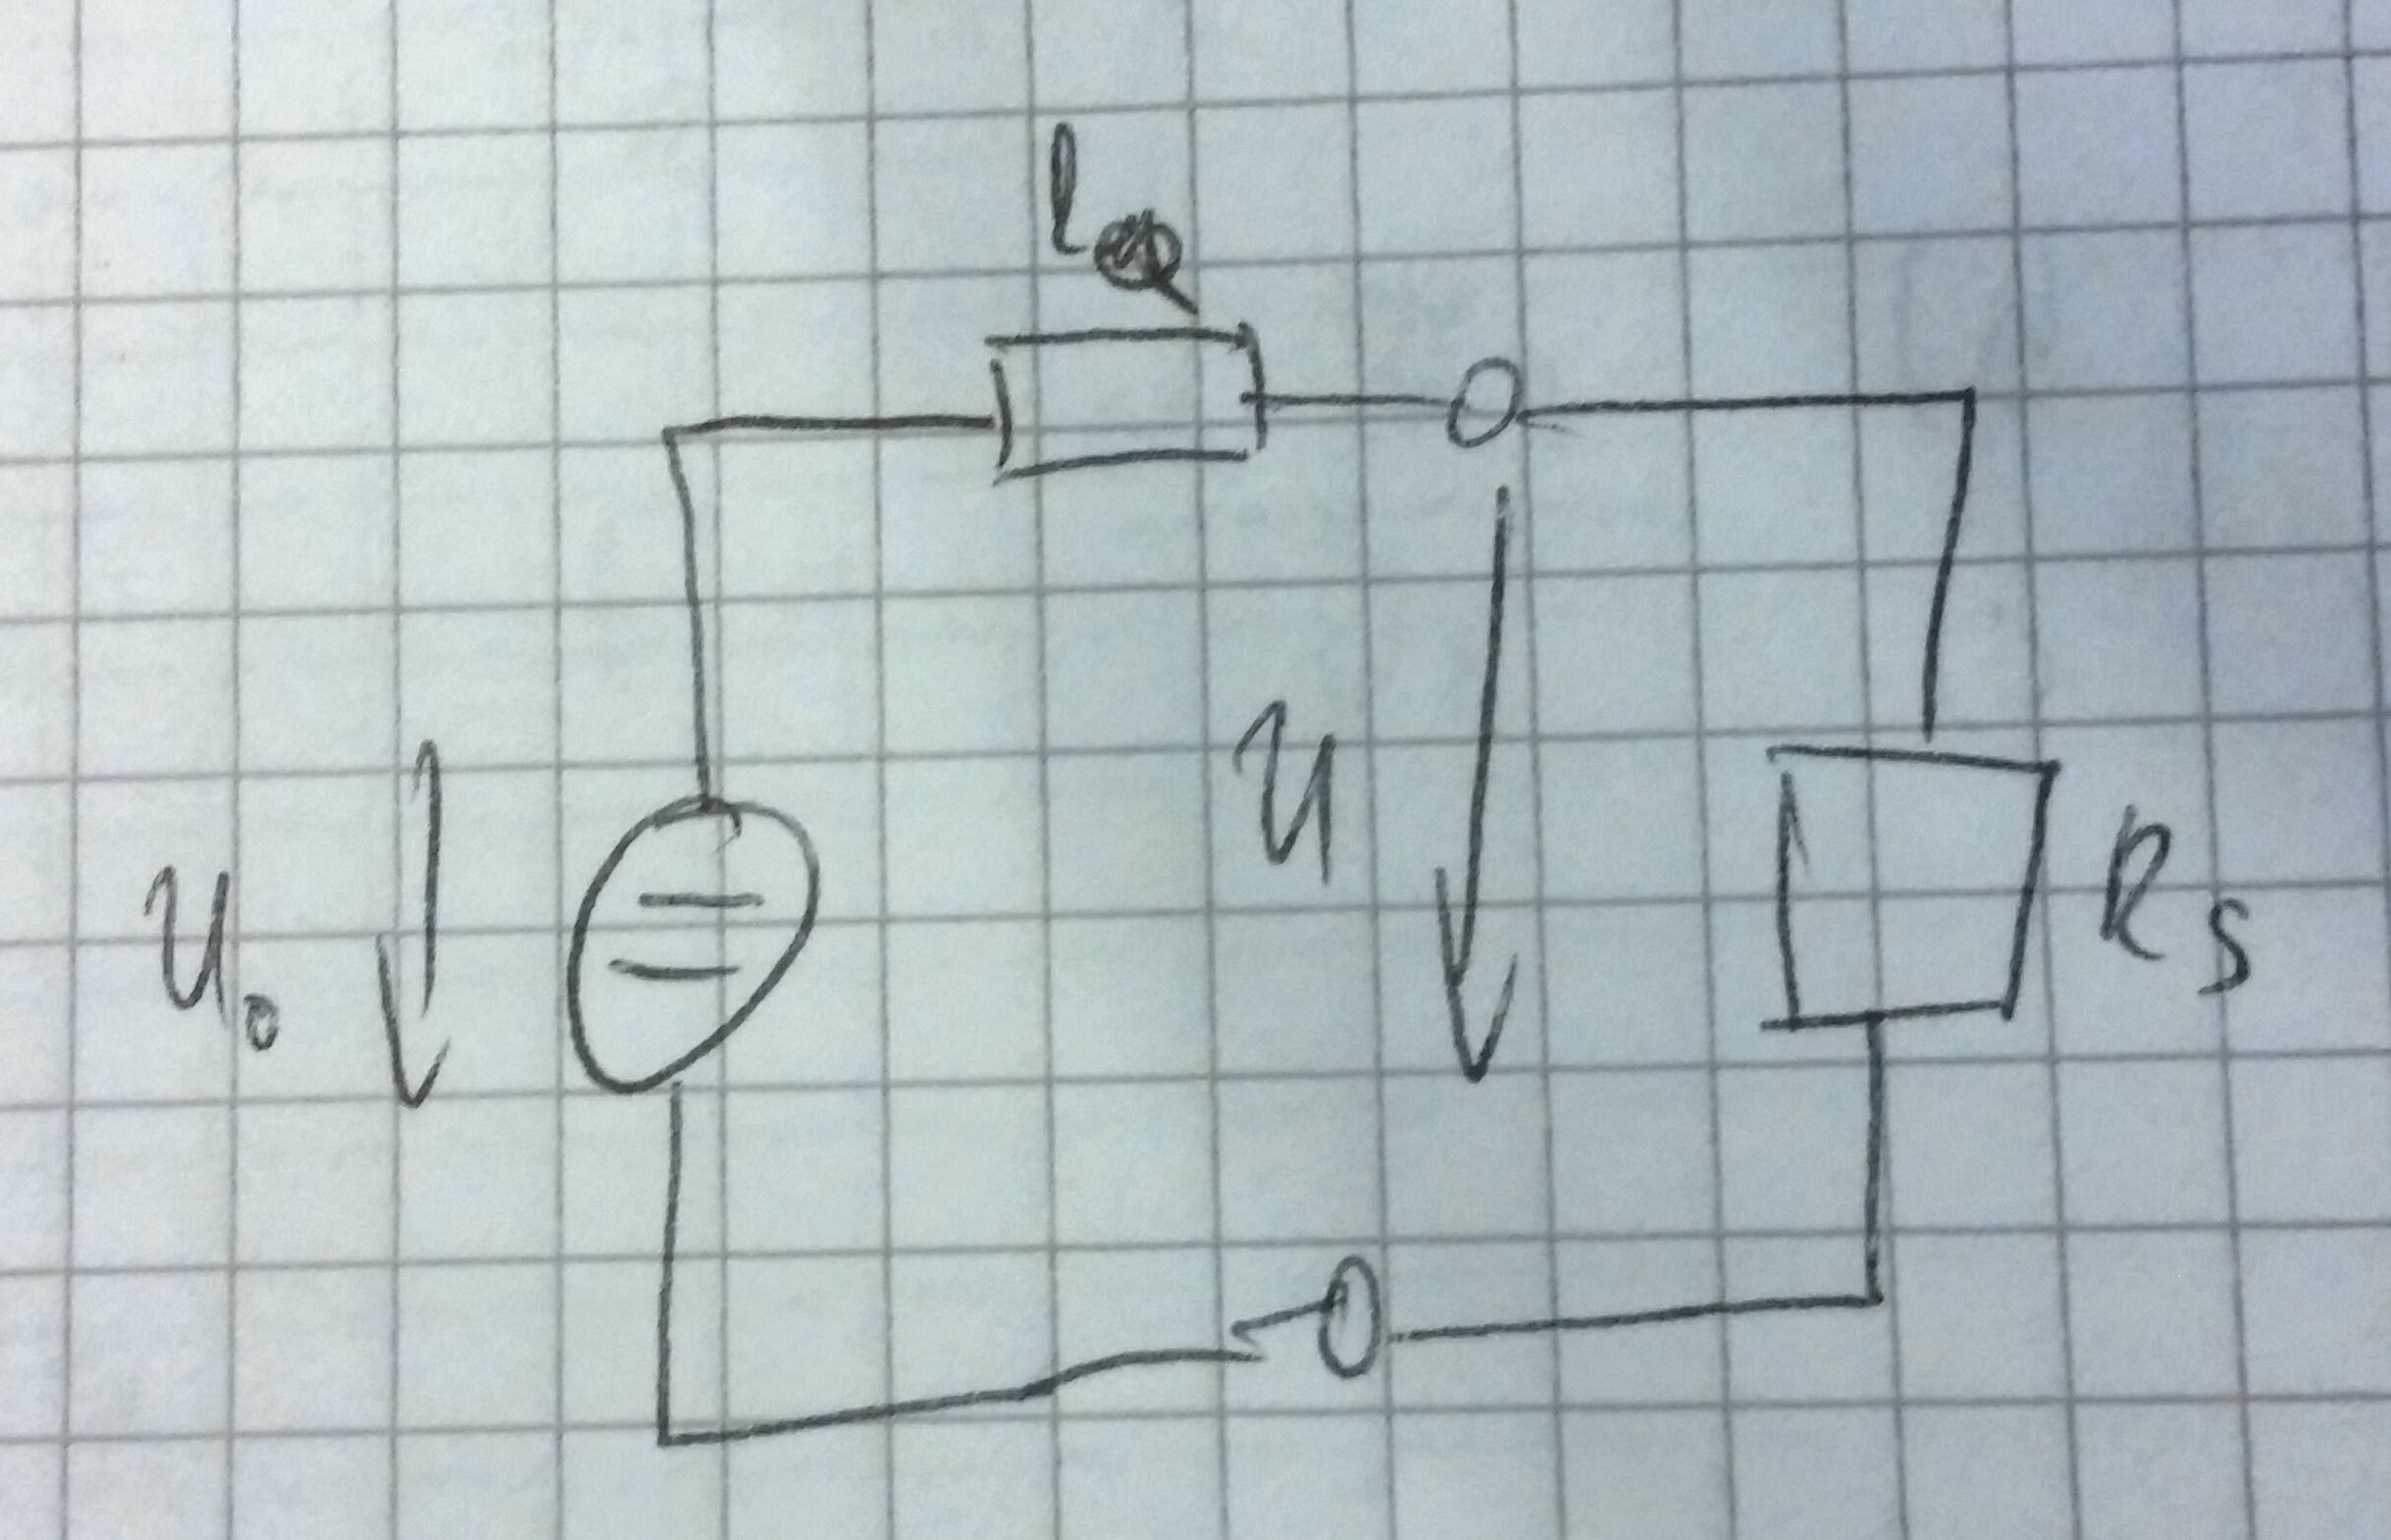
\includegraphics[scale=0.15]{A3_1.jpg}
\end{figure}




\begin{align*}
I = \frac{U_0}{R_Q + R_S} \leq I_K = \frac{U_0}{R_Q}
\intertext{$R_S$ darf nur \unit[1]{\%} von $R_Q$ betragen:}
R_S \leq 0,01 \cdot R_{Q,min} = 0,01 \cdot \unit[0,2]{\Omega} = \unit[0,002]{\Omega}
\end{align*}


\subsection*{b)}

Wir nutzen die Spannungsteilerregel:

\begin{align*}
\frac{U_S}{U_0} &= \frac{R_S}{R_Q + R_S} \\
\Leftrightarrow U_S &= \frac{0,002}{0,3 + 0,002} \cdot 10 = \unit[0,066]{V}
\end{align*}


\subsection*{c)}

\begin{align*}
P &= \frac{U^2}{R} = \frac{0,066^2}{0,002} = \unit[2,19]{W}
\end{align*}

Das ist bei einem so kleinen Bauteil schon eine nicht zu vernachlässigende Verlustleistung.


\subsection*{d)}


Der Shuntwiderstand wird durch die Leistung $P$ erwärmt. Da $R$ von der Temperatur $T$ abhängt kann es zu einer Fehlmessung kommen.


\section{Aufgabe 4}

\subsection*{a)}

\subsubsection*{Aktiv}

\begin{align*}
\frac{U_2}{U_1} = \frac{R_2}{R_1} \cdot \frac{1}{1 + j \omega R_2 C}
\end{align*}


\subsubsection*{Passiv}

\begin{align*}
\frac{U_2}{U_1} = \frac{\frac{1}{j \omega C_2}}{R_2 + \frac{1}{j \omega C_2}} = \frac{1}{1 + j \omega R_2 C_2}
\end{align*}


\subsection*{b)}

\begin{align*}
V &= 10^{\frac{26}{20}} = 19,95 \approx 20 \\
V &= \frac{R_1}{R_2} \\
\Leftrightarrow R_2 = 19,95 \cdot R_1 = \unit[199,5]{k \Omega}
\end{align*}


\subsection*{c)}

\begin{align*}
T &= R_2 \cdot C_2 = \frac{1}{\omega} = \frac{1}{2 \pi f} \\
\Leftrightarrow C_2 &= \frac{1}{2 \pi f \cdot R_2} = \frac{1}{2 \pi \cdot 100 \cdot 199,5 \cdot 10^3} = \unit[7,98]{nF}
\end{align*}


\subsection*{d)}

\begin{itemize}
	\item Verstärkung
	\item Eingangsimpedanz ist frequenzabhängig
	\item Ausgangimpedanz ist frequenzabhängig
\end{itemize}



















\end{document}